\chapter{强化学习方法}
延迟敏感型任务和批处理任务的混合执行能显著提高服务器的资源利用率。气泡测试等方法也使得我们能够以可接受的代价确定合适的混合策略。借助上文提到的基于硬件或软件的资源隔离方法,延迟敏感型任务的服务质量可以得到有效保证。然而,对混合执行任务使用静态的资源分配方案无法充分得利用服务器资源\---任何的静态的资源分配要么过于保守,导致资源利用率不足;要么过于乐观,导致延迟敏感型任务违反其服务质量要求\cite{lo2015heracles}
\section{动态资源调度的动机}
当两个或多个任务并行执行时,任务之间竞争共享的资源。硬件和软件上的资源隔离技术使得我们能够在一定程度上控制这种竞争,以减少不同任务之间的相互影响。本节分析混合执行中存在的主要资源竞争,以及进行动态资源管理的动机。

\subsection{处理器核心}
单个服务器中最主要的共享资源是一个或多个处理器接口中的处理器核心。我们不能简单的通过cgroup等工具将计算核心按统计学指标静态地分配给延迟敏感型任务和批处理任务。当延迟敏感型任务,例如搜索引擎,达到吞吐量高峰时,需要所有可用的核心来满足负载需求以避免违反服务质量要求。仅仅给延迟敏感型任务分配更高的进程调度优先级并不能解决问题。例如Linux系统的完全公平调度器(Completely Fair Scheduler, CFS)在内的常见调度器由于算法的缺陷,在延迟敏感型任务和批处理任务混合执行时常常导致延迟敏感型任务违反服务质量要求\cite{leverich2014reconciling}。实时调度算法,例如Linux的SCHED\_FIFO并不保存已完成的运算,导致系统资源实际利用率下降。

\subsection{末级高速缓存}

当混合执行的任务中含有面向用户的延迟敏感型任务时,末级高速缓存的动态管理更加重要。延迟敏感型任务的缓存占用随着其负载强度的变化而产生改变\cite{leverich2014reconciling},与此同时,其对批处理任务通过共享末级高速缓存引起的干扰的敏感程度,也因自身的负载强度也有所不同。当延迟敏感型任务处于高负载状态时,轻微的相互干扰会引起巨大的延迟\cite{kasture2014ubik},例如Google的机器学习中的聚类任务(ml\_cluster)在负载50\%左右时基本不受来自末级高速缓存压力的影响,但在更高的负载强度时对其干扰十分敏感\cite{lo2015heracles}。

过量限制批处理任务利用末级高速缓存并不能有效保证延迟敏感型任务的服务执行,也不一定利于提高服务器的资源利用率。一些批处理任务对末级高速缓存大小变化敏感,当可用缓存大小减少,其缓存不命中率可能迅速升高,导致其对动态随机存储的访问次数上升,处理器将花费更多时间等待数据的输入输出,导致批处理任务性能降低,服务器资源实际利用率降低。更糟糕的是,批处理任务的缓存不命中率上升同时还将使其占用更多访存带宽,降低延迟敏感型任务访问动态随机存储器的性能,从而影响其服务质量。通过英特尔提供的内存带宽监控技术(MBM)和内存带宽分配技术(MBA)可以减轻此问题的影响,然而目前仅有少量最新的处理器硬件支持此技术。

当混合执行的任务中包含面向用户的延迟敏感型任务时,延迟敏感型任务对末级高速缓存占用随负载强度的动态变化,其处于高负载状态时对末级高速缓存压力的敏感程度和多种共享资源占用的相互干扰,体现出动态分配末级高速缓存以满足不同负载时的资源需求的必要性与确定合理动态分配末级高速缓存策略的难度。


\subsection{网络带宽}
数据中心的大型应用程序主要是通过向外扩展(scaling-out)达到其规模,因此服务器之间的网络连接性能也至关重要。因为延迟敏感型任务产生的网络流量随负载强度变化,网络带宽的管理也应动态进行。静态的优先级设置会导致网络连接的低利用率和批处理任务的饥饿(starvation)\cite{pattara2002starvation}。对网络带宽的动态管理也可以延伸至对固态存储器(Solid State Storage)访问带宽的管理上\cite{seong2010hydra}。

\subsection{热功率}
因处理器总体热设计功耗(Themal Design Power)限制,同一处理器接口上的核心之间会相互影响其最大时钟频率,进而影响计算性能。为保证运行延迟敏感型任务的核心不会因为运行批处理任务核心过度能耗使用而导致时钟频率的突然下降,必须限制运行批处理任务核心的时钟频率。静态将运行批处理任务的核心设置在最低时钟频率可以避免运行延迟敏感型任务的核心因能耗而被限制性能。然而使用静态的设置严重影响了批处理任务运行的性能。大部分的批处理任务并不总是会使核心处于高能耗状态,并且延迟敏感型任务也仅仅在高负载强度时才需要提升核心频率来获得额外的性能提升。为了在保证延迟敏感型任务在高负载时获得合理的时钟频率的同时,尽可能避免过分限制批处理任务的性能,动态的核心热功率控制是必要的。

\section{动态资源调度于强化学习}
混合执行延迟敏感型任务和批处理任务的更大挑战在于控制两种任务同时在上述多种资源上复杂的相互干扰。批处理任务会同时在各种共享资源上对延迟敏感型任务产生干扰,而延迟敏感型任务对来自各种共享资源上的干扰都十分敏感。因此,仅仅控制好一种共享资源上的相互干扰是不足以保证延迟敏感型任务的服务质量的;所有共享资源都应尽可能的监控并有效的实施干扰隔离。除此之外,各种共享资源上的干扰还会相互影响。例如,延迟敏感型任务和批处理任务在缓存上的竞争会导致某一任务对动态随机存储访问带宽的要求提高,成为潜在的性能瓶颈;又例如当任务检测到网络连接拥塞,将可能会采取更激进的压缩算法,导致计算资源和能耗的竞争。各种资源的相互竞争导致难以在保证延迟敏感型任务的服务质量的同时,通过动态资源调度提升服务器资源利用率。

\begin{figure}
  \centering
  \begin{minipage}[b]{0.7\textwidth}
    \centering
    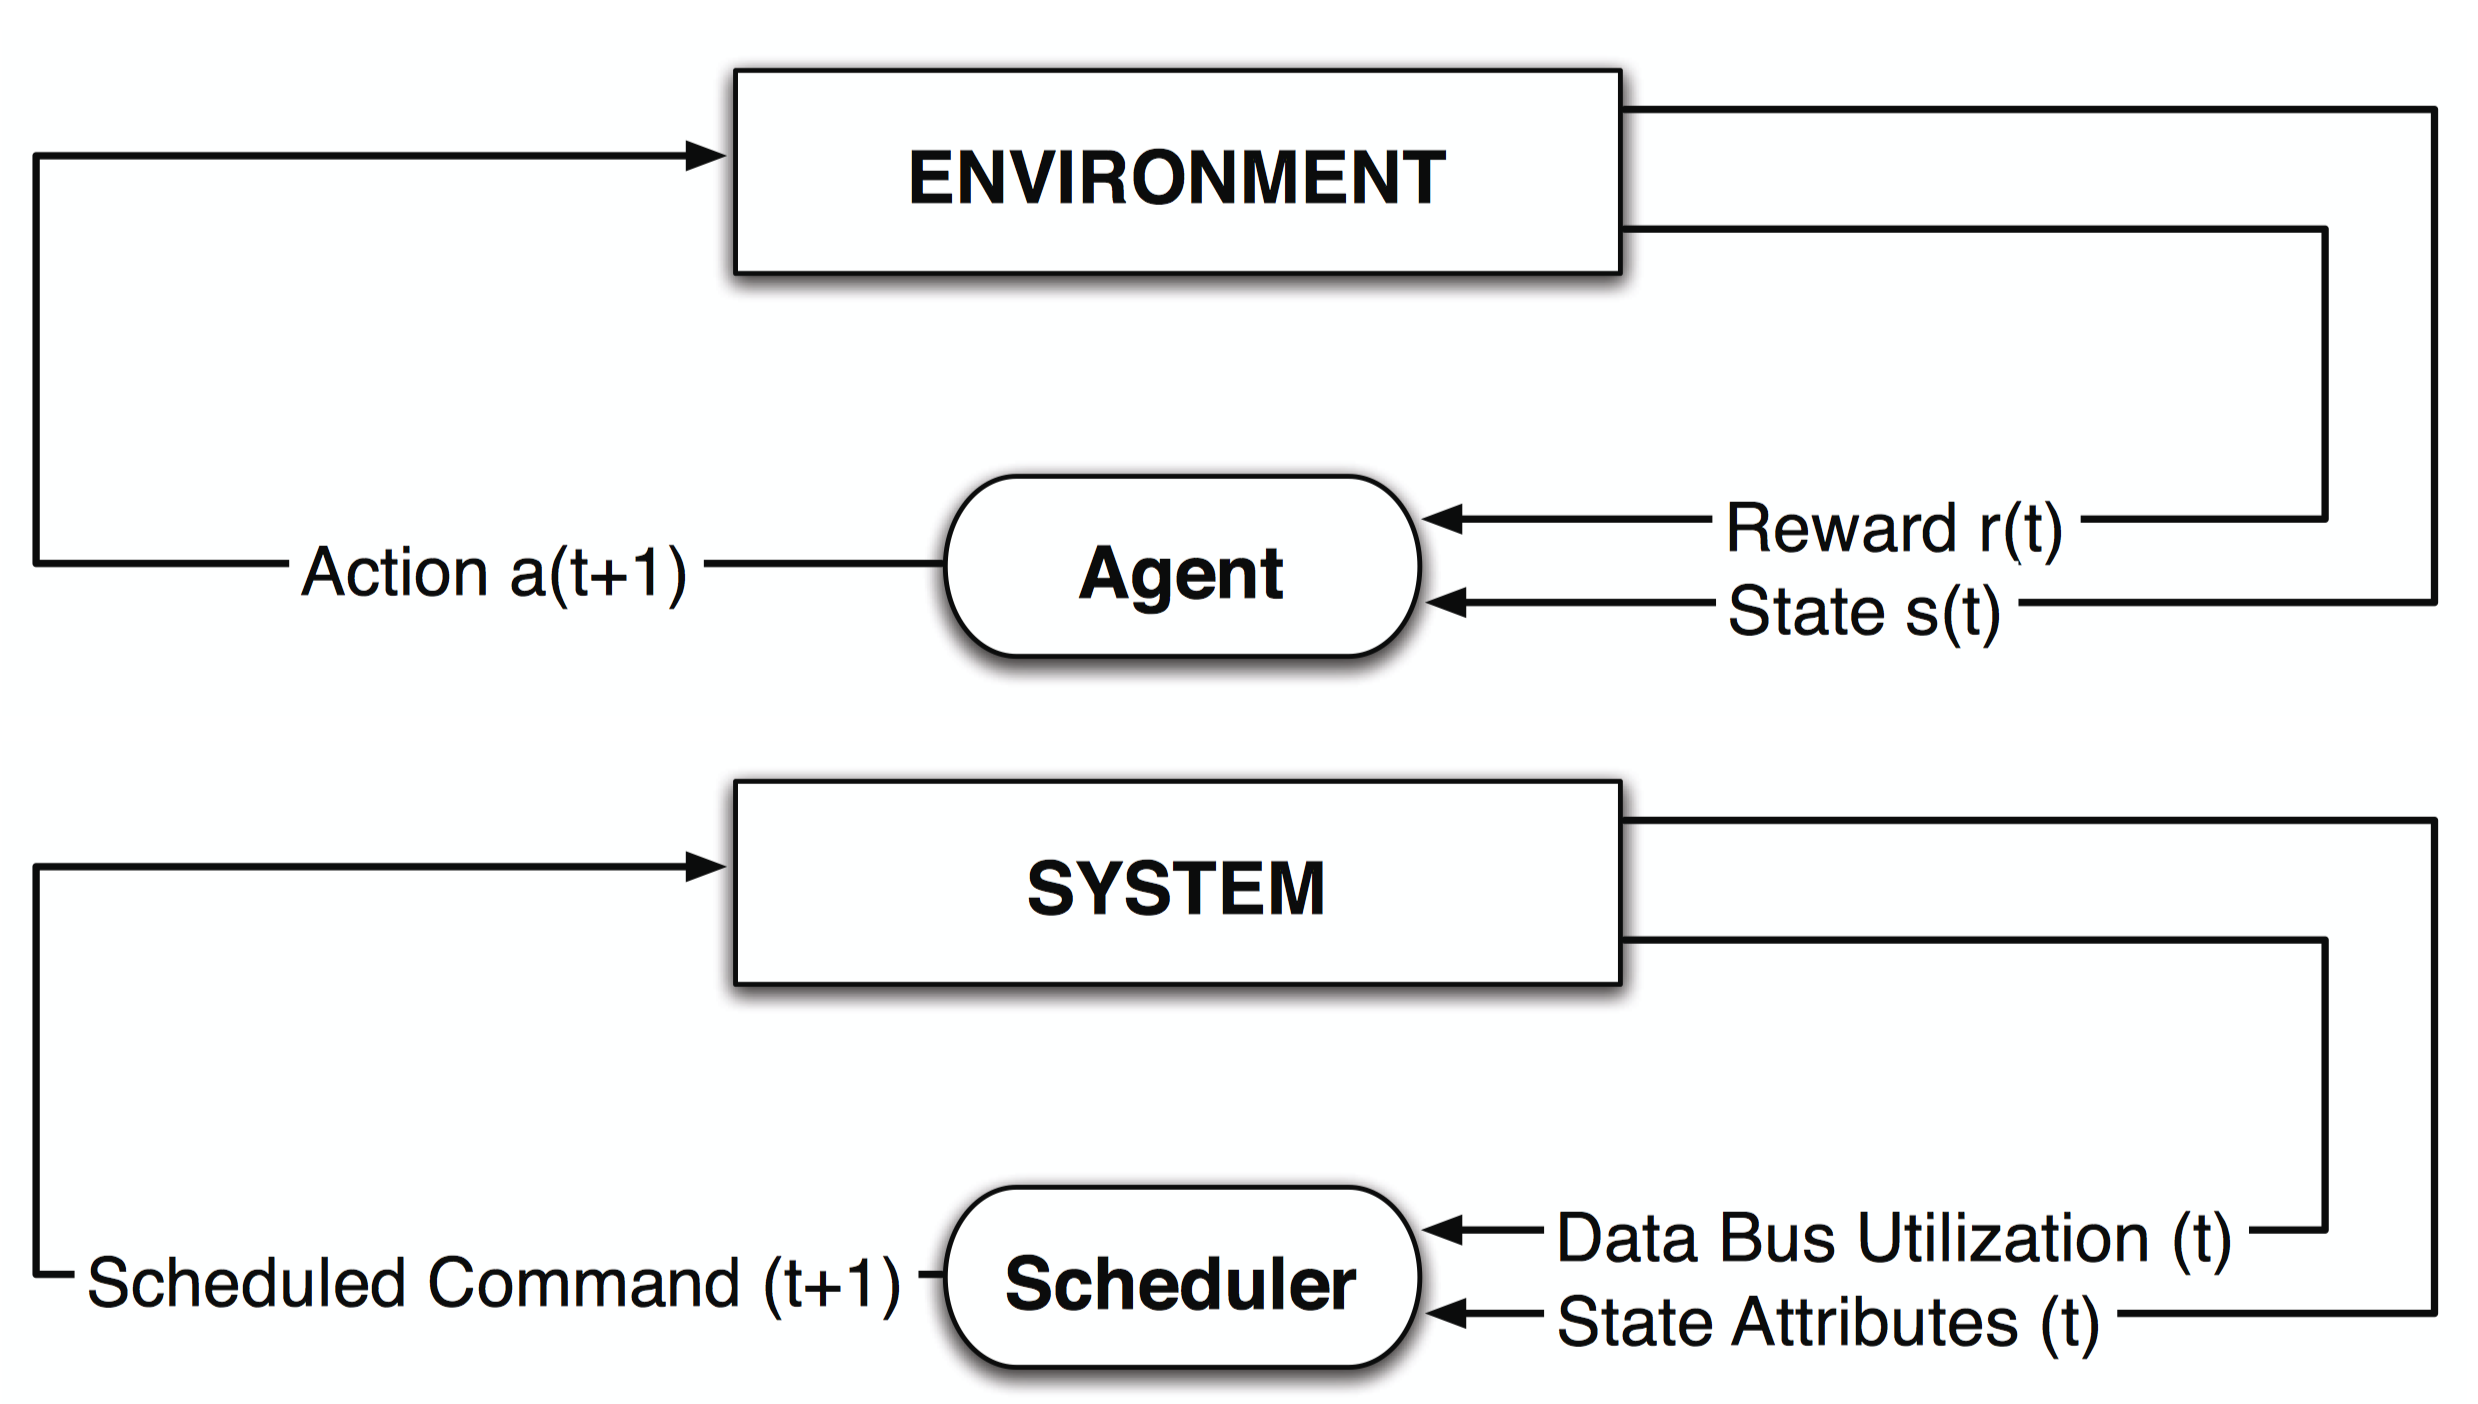
\includegraphics[width=1\linewidth]{rl/rl.png}
    \captionof{figure}{强化学习框架}
    \label{fig:rl}
  \end{minipage}     
\end{figure}


强化学习在一些极具挑战性的决策类优化问题中表现出其巨大潜力\cite{mnih2013playing}\cite{silver2016mastering}。强化学习中,智能体(agents)从过往的经验学习以做出更好的决策。图\ref{fig:rl}(a)展示了智能体如何与环境交互。交互过程被离散化成为一连串步骤,每一步智能体先感知环境的状态(state)为$s_t$,然后选择并执行一个动作(action)。这一步骤将导致环境的状态发生变化,转移至$s_{t+1}$,智能体在后续步骤中也将能够感知,此状态的变化还将生成一个奖励信号(reward)$r_t$。智能体对任务本身和规则一无所知,仅仅通过环境返回的奖励信号来的得知他当前学习到策略的好坏\cite{bertsekas1995dynamic}。智能体学习的目标时通过优化自身选择动作的策略,以最大化其累积奖赏。强化学习最近的研究将其和深度学习相结合,使得强化学习在很多应用上取得突破性的成绩,比如玩电子游戏\cite{mnih2015human},控制数据中心的冷却系统\cite{evans2016deepmind}等等。

回顾优化数据中心资源调度的问题,我们相信强化学习非常适合解决此类问题。首先,资源调度程序做出的决策通常有很高的重复性,因此可以产生大量数据用于强化学习训练。其次,正如我们在强化学习算法应用在游戏\cite{mnih2015human}\cite{evans2016deepmind}时看到的,强化学习算法可以通过深度神经网络(Deep Neural Network, DNN)模拟复杂的模型和决策过程。不同的信号和环境可能存在的轻微扰动都可以整合起来同时输入神经网络,产生一个决策模型。另外,通过强化学习,我们能够通过一个相关的奖励信号来优化一些难以直接优化的目标。最后,通过持续的学习,强化学习可以从大量经验中学到不同情况下的优化策略。

图\ref{fig:rl}(b)展示了如何在强化学习的框架内优化数据中心的资源调度以提高服务器利用率。智能体在这里充当资源调度器,而环境则包含了混合执行的延迟敏感型任务和批处理任务,支持这些任务的执行的所有服务器资源,以及按一定模式变化的延迟敏感型任务的负载。强化学习的每一步骤对应资源调度器的一次决策,智能体将在此时获得环境的状态并做出动作。环境相关的信息包括当前延迟敏感型任务的负载强度,计算核心,末级缓存和随机存储访存带宽等等资源的利用率,以及延迟敏感型任务的服务质量。智能体可做的选择则为增加分配给延迟敏感型任务的某类服务器资源,以提高其服务质量并避免违反服务质量要求,或是减少分配给延迟敏感型任务的某类资源以提高批处理任务性能并提高资源利用率。环境产生的奖励信号有多种设计目标。若此动作的执行导致资源敏感型任务违反其服务质量要求,智能体将给予惩罚(负的奖励);在不违反服务质量要求时,延迟敏感型任务占用的资源越少,智能体收到的奖励越大;所有的动作并不都一定可以在任意环境状态下执行,例如某类资源分配无法增加或减少,智能体若做出非法动作将会受到惩罚。

\section{强化学习在资源调度中的挑战}
将强化学习应用在数据中心的资源调度上时,同样面临挑战。首先是功劳分配问题(Temporal Credit Assignment),智能体需要学习如何从直接观察到的奖励信号中分析以前所执行的动作哪些有正面的贡献,哪些产生了负面的影响,以及这些负面的贡献和影响各有多大。在一些情况中,一些能立即产生高额奖励的动作可能将使系统进入不理想的状态,难以产生更多的奖励;而另一些情况中,一个动作可能无法产生立即的奖励,但可能对系统进入一个理想状态至关重要。因此最优的策略需要产生长远的规划,智能体需要能够预见未来的可能情况才能采取相应的行动以最大化总的奖励。其次是探索环境的积极性。智能体需要探索环境,学习不同状态下执行不同动作所带来的后果。一方面,积极的探索环境让智能体可能学会更高效的控制策略;另一方面,智能体在任何时刻也应该尽量执行已经找到的最优策略。对环境的探索太少将导致智能体始终执行没有足够优化的策略;而过多的探索将使智能体长时间执行不够优化的策略,拉长训练时间,且降低其性能表现。最后是泛化问题,环境的状态空间随考虑的因素指数增长,表示环境状态的变量可能相当大。在这种情况下,智能体很可能根本无法在此遇到以前经历过的环境状态。因此,从智能体的经验中学习并泛化是唯一可行办法。

\section{强化学习方法简介}
\subsection{马尔科夫决策过程(Markov Decision Processes, MDPs)}
考虑一般的强化学习场景,如图\ref{fig:rl}(a)所示,在每一步骤$\mathrm{t}$能观察到环境状态$\mathrm{s_t}$。当智能体执行动作$\mathrm{a_t}$后,环境状态变为$\mathrm{s_{t+1}}$,且智能体收到奖励$\mathrm{r_t}$。环境状态的转变和智能体收到的奖励都是随机的,并被假设具有马尔科夫性质(Markov Property)。因此,智能体所处的环境被抽象为马可夫决策过程(Markov Decision Processes,MDPs)。一个马尔科夫决策过程包含了一个状态集合$\mathbb{S}$,一个动作集合$\mathbb{A}$,一个状态间转换的关于动作的条件概率分布$\mathrm{T=\mathbb{P}(s_{t+1}=s'|s_t=s, a_t = a)}$,以及在每个状态下执行一个动作使得环境状态改变至另一个状态的奖励的期望$\mathrm{R=\mathbb{E}[r_t+1|s_t=s, a_t=a, s_t+1=s']}$。

\begin{figure}
  \centering
  \begin{minipage}[b]{0.7\textwidth}
    \centering
    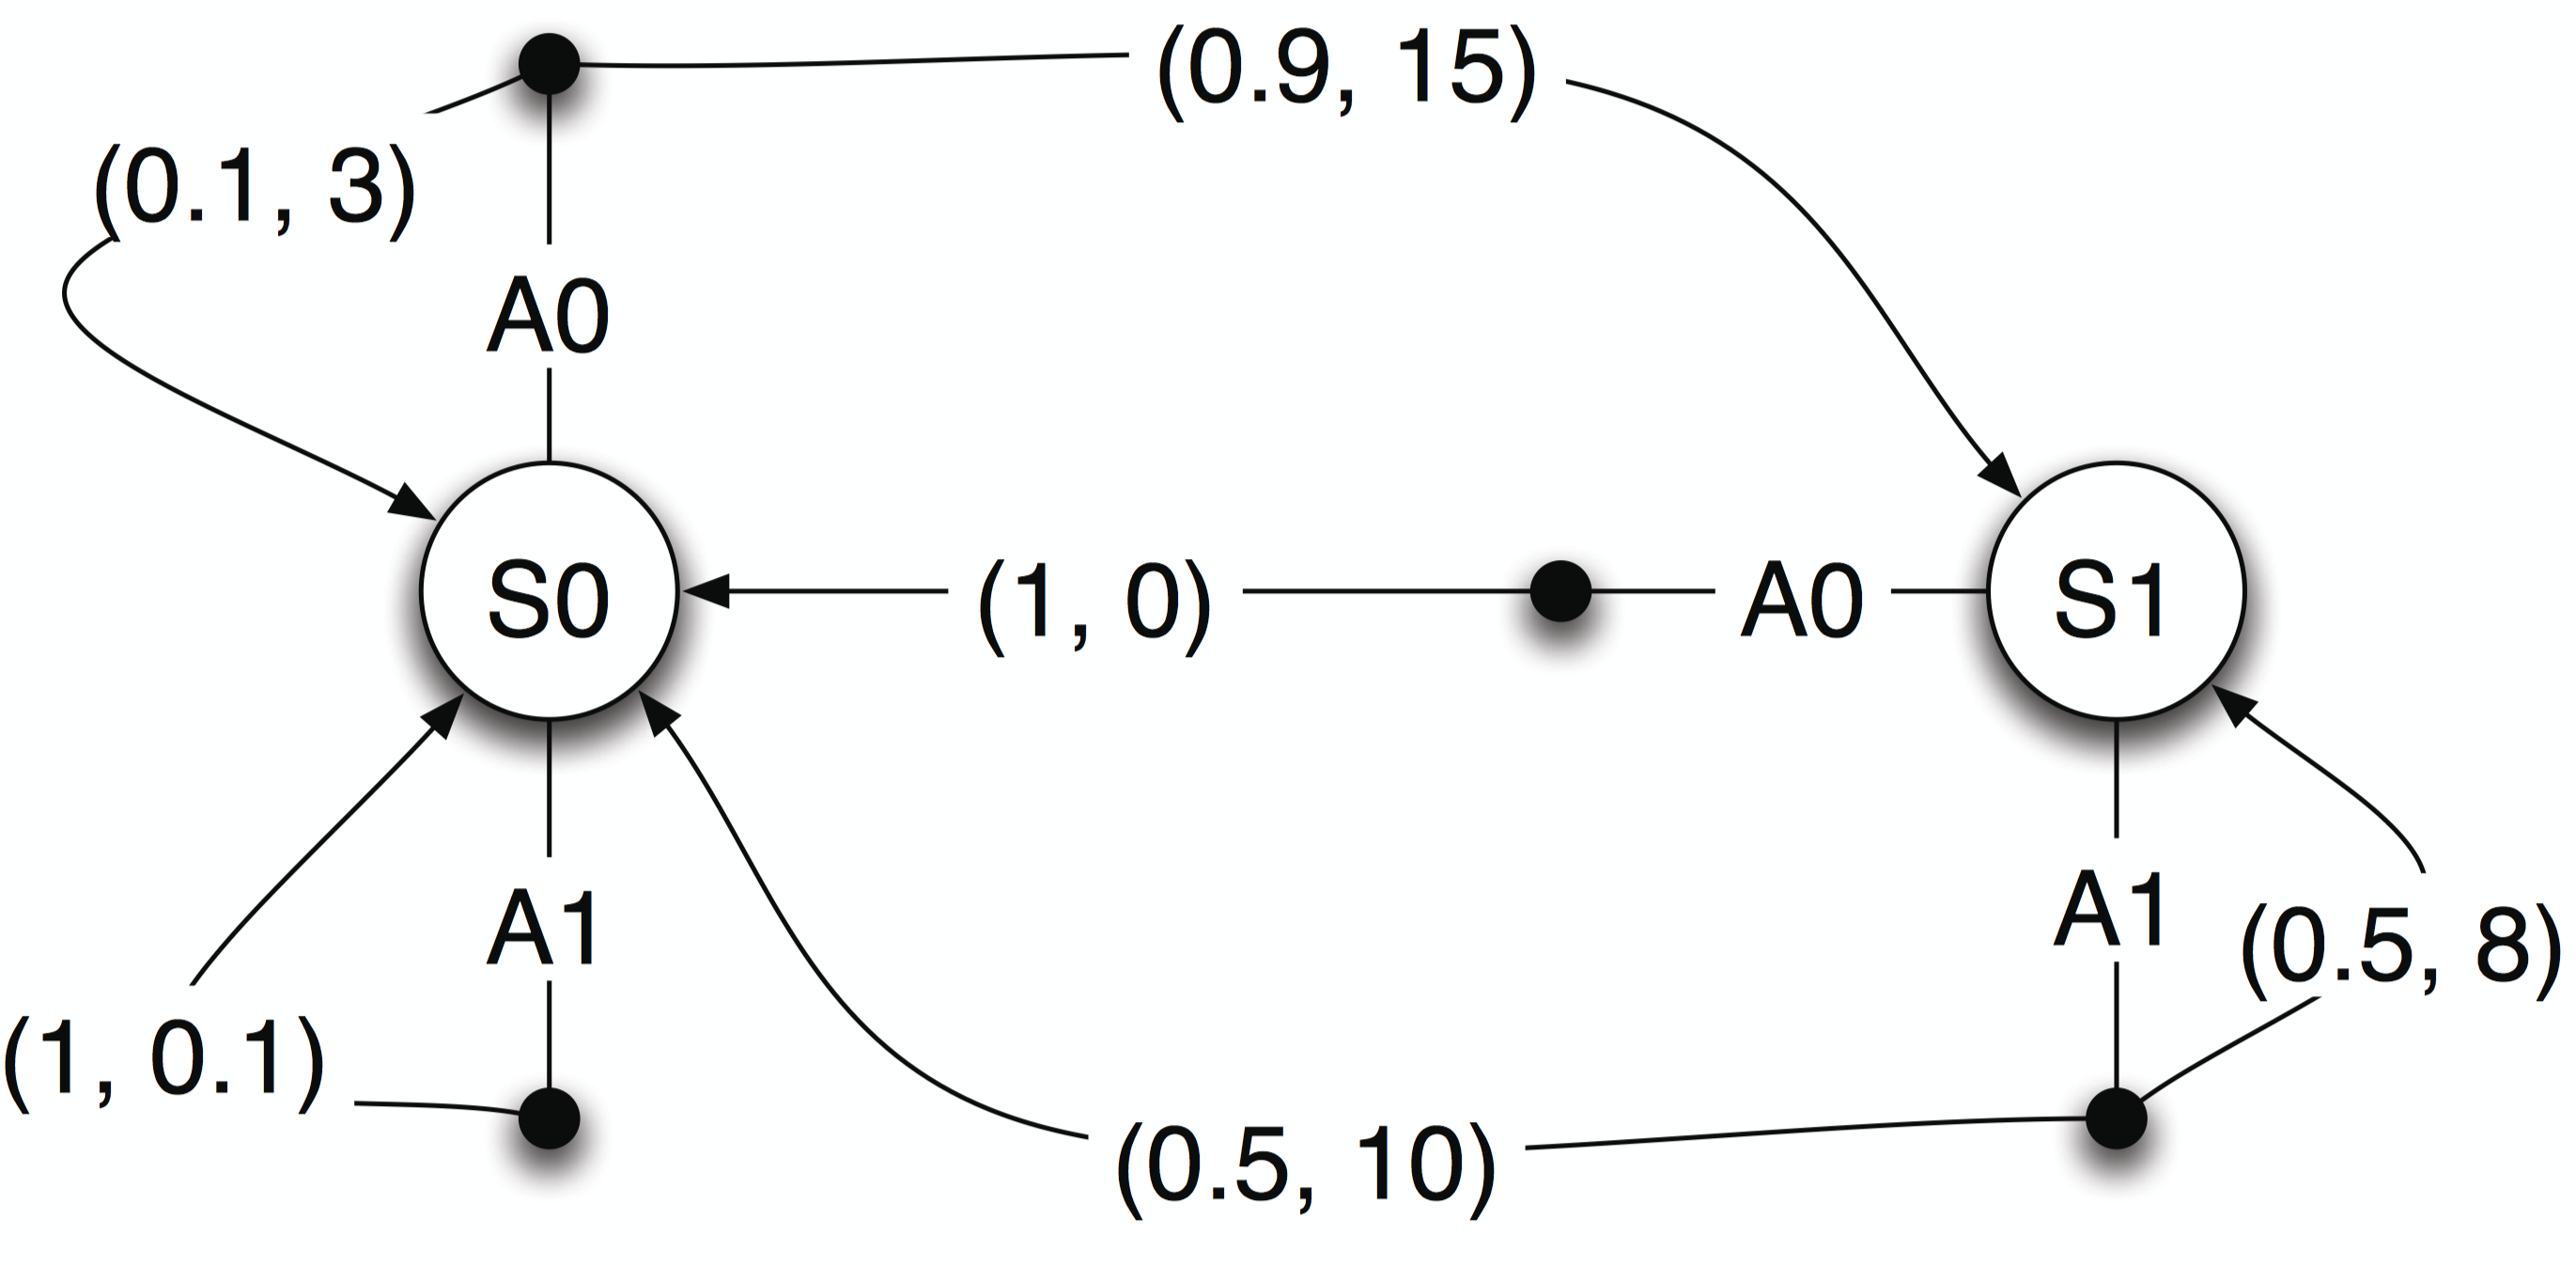
\includegraphics[width=1\linewidth]{rl/mdp.png}
    \captionof{figure}{马尔科夫决策过程示例}
    \label{fig:mdp}
  \end{minipage}     
\end{figure}

图\ref{fig:mdp}是一个马尔科夫决策过程的示例。示例的马尔科夫决策过程定义了两个环境状态$S0$和$S1$,和智能体在两个状态下都可选择执行的两个动作$A0$和$A1$。智能体在状态$S0$下执行动作$A0$,有$0.1$的可能性留在状态$S0$并获得$3$的奖励;同时有$0.9$的可能性转移至状态$S1$并获得$15$的奖励。智能体能控制的仅仅是选择下一个执行的动作,并且对环境可能的反应没有任何先验的知识。因此智能体的目标在于优化自身选择动作的策略以获得最大的累积奖赏。值得注意的是,对于智能体来说,执行某一动作后的状态转变并不总是确定的,有时是按概率跳转的。环境状态如何变化不在智能体的控制范围内,但智能体能通过大量的经验学习到其变化的规律。

用强化学习框架解决资源调度问题时,很自然会将总的步骤设为无限步骤,在无限长的时间里智能体通过合理分配服务器资源给延迟敏感型任务以保证其服务质量要求同时尽量提高服务器资源利用率。随着智能体考虑的时间由有限变为无限,一个潜在的问题是劣质的策略也能带来无限的总效用,导致智能体无法定义一个有效的优化目标。因此,在无限时间步骤时,优化折现后的累计奖赏(discounted cumulative reward)更为合适,这可以理解为如果能拿到奖赏,智能体倾向于尽早拿到奖赏。同时,由于智能体的优化目标仍然是累积奖赏,因此智能体仍然有发现远期更高价值奖赏的潜力。折现累积奖赏可表示为\ref{eq:discounted_reward},其意义为当前步骤后执行$i$次动作后得到奖赏的期望$r_{t+i}$在当前决策中的价值为$\gamma^i*r_{t+i}$,其中$\gamma$为折现率。

\begin{equation}
  \label{eq:discounted_reward}
    R = \mathbb{E}(\sum_{i=1}^{\infty} {\gamma^{i}} \cdot r_{t+i})
\end{equation}

\subsection{策略与状态值函数}
强化学习中智能体根据其学习到的策略和观察到的环境状态选择下一执行动作。策略是一个关于动作的条件概率$\pi: \pi(s, a)\rightarrow[0,1]$。$\pi(s, a)$表示了智能体在环境状态为$s$时选择执行动作$a$。当考虑的环境因素增加时,环境状态的可能情况呈指数上升。一般具有时间研究意义的问题都考虑较多的环境变量导致环境状态空间巨大。这种情况下,智能体学习的策略无法用传统的表格方式表示,而需要用一个函数来近似\cite{bertsekas1995dynamic}\cite{menache2005basis}。通过函数近似,我们可以用可接受数目的参数$\theta$来近似策略$\pi(s, a)$,我们将通过参数$\theta$来参数化近似表示的策略记为$\pi_\theta(s,a)$。函数近似可以解决问题的一个理由是对于相似的状态,我们认为智能体本来也应该采取相同的动作以优化其目标。

很多函数近似方法都可以用来实现近似强化学习中的策略函数,例如通过环境状态和动作空间的特征进行线性组合来近似策略$\pi(s,a)\approx\pi_\theta(s,a)=\theta^T\phi(s,a)$。 深度神经网络在最近的研究中被用作函数近似来表示策略函数,并在一些大规模的强化学习场景中取得很好效果。使用深度神经网络而不是前文提到的特征的线性组合的一个优点是不需要繁琐的特征工程来选取环境状态和动作中的特征。图\ref{fig:policy}表示了如何使用深度神经网络来近似策略函数时进行强化学习。

\begin{figure}
  \centering
    \centering
    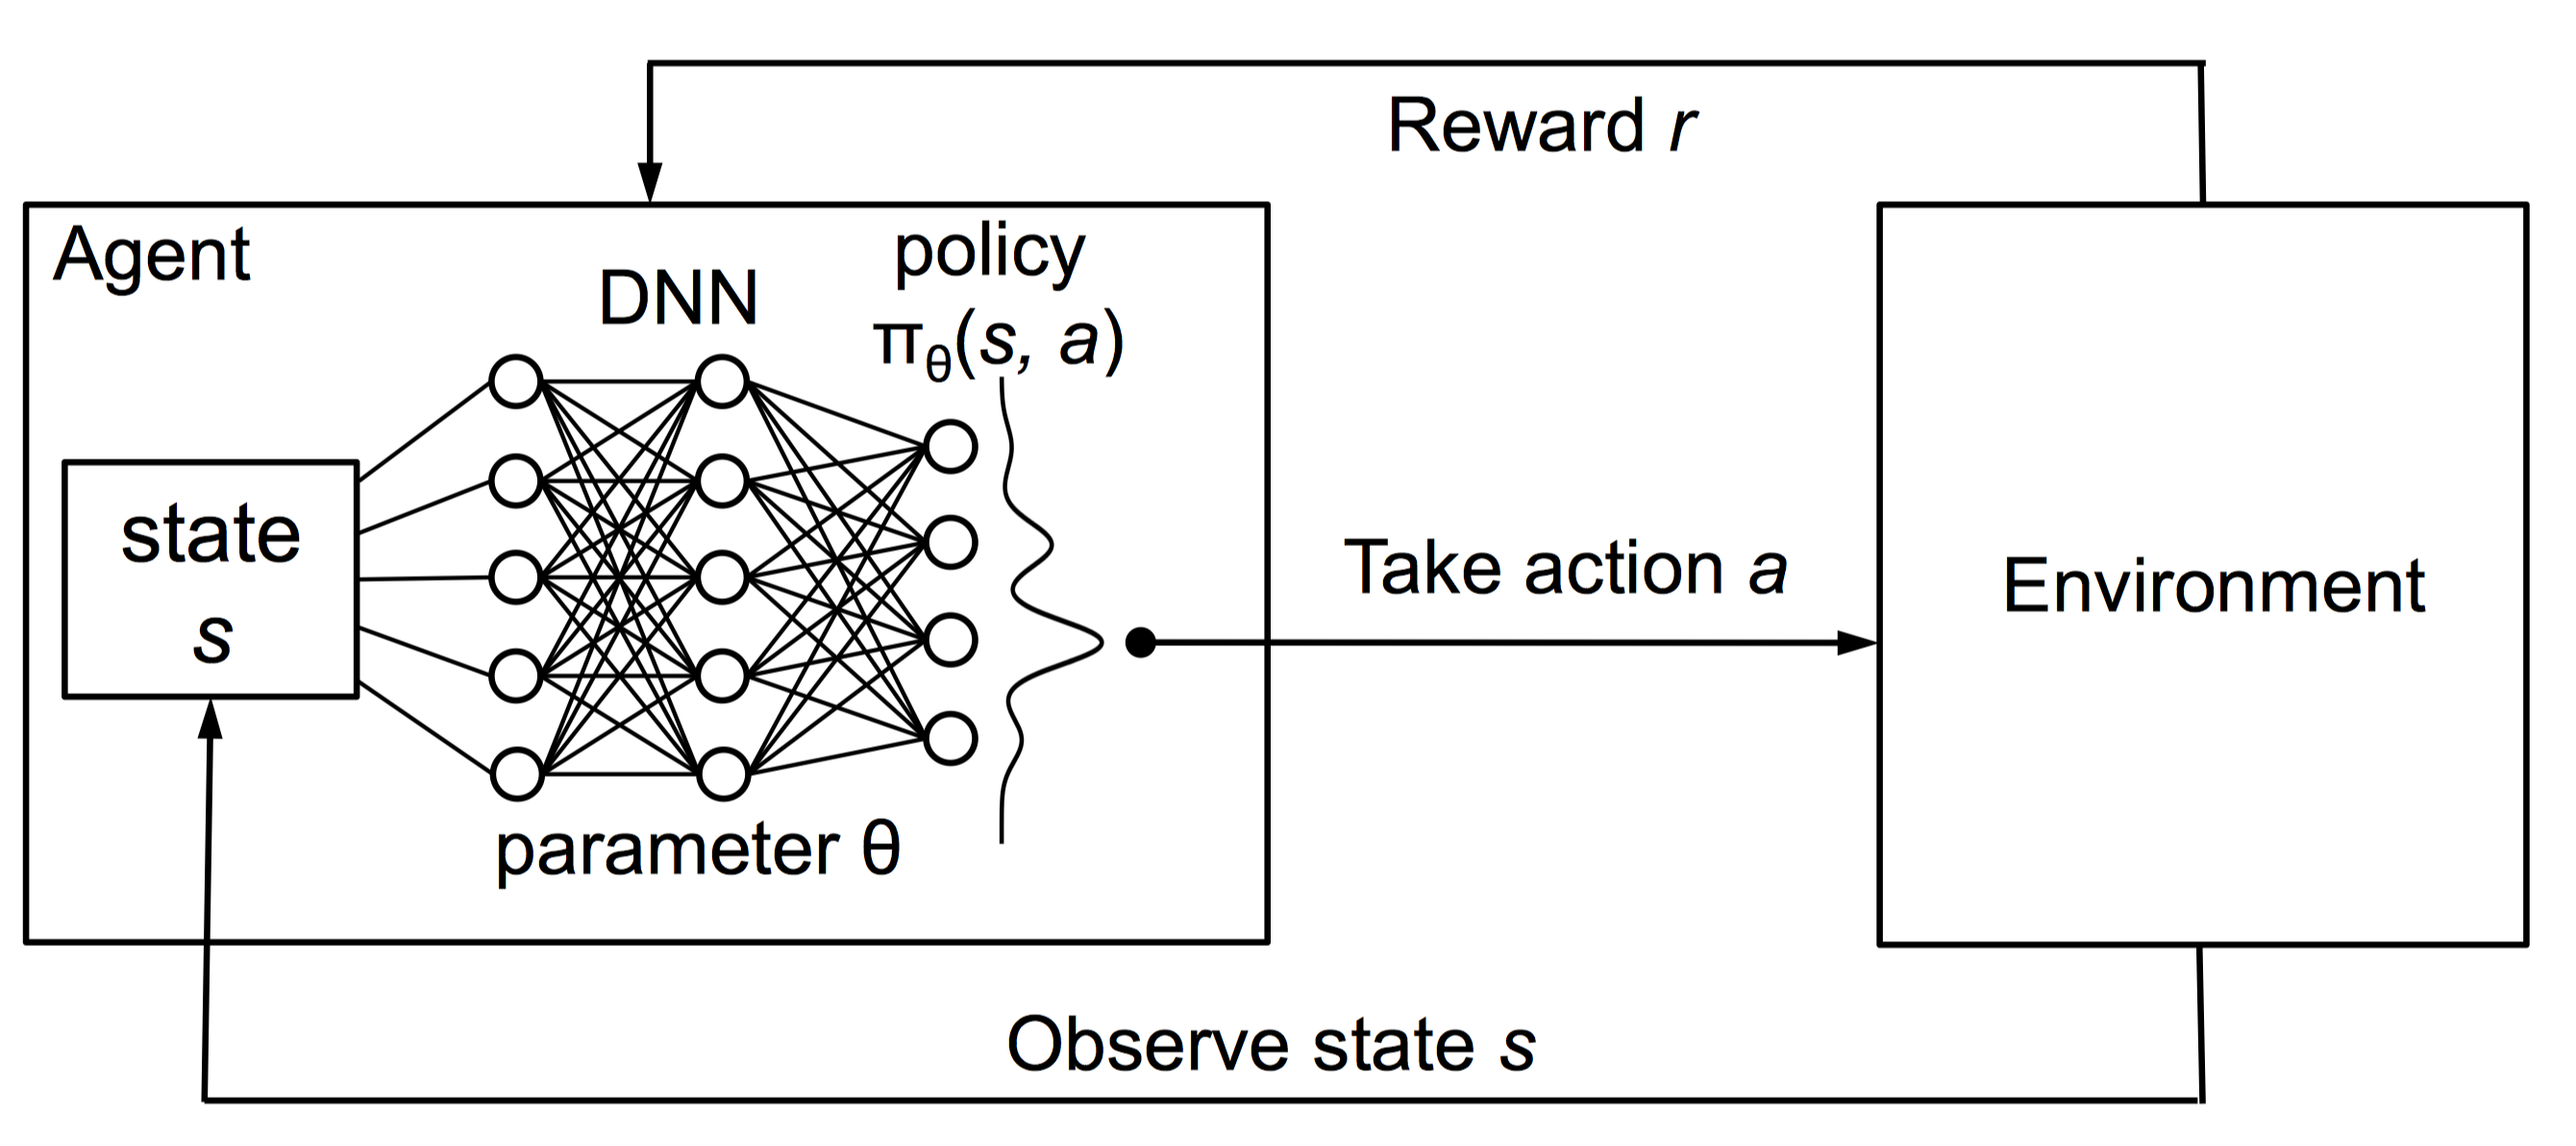
\includegraphics[width=1\linewidth]{rl/policy.png}
    \captionof{figure}{通过深度神经网络近似策略函数}
    \label{fig:policy}    
\end{figure}

当智能体按照一个给定的策略选择动作并执行时会产生一系列的环境状态,执行动作和奖赏信号的序列,如$s_0, a_0, r_0,s_1, a_1, r_1 ...$。状态值函数(Value Function),见式\ref{eq:val_func},$V^{\pi_\theta}(s)$表示了从指定的环境状态$s$开始,执行按照策略$\pi_\theta$产生的动作序列,可获得的折现后累积奖赏的期望。我们将状态值函数,作为判断一个环境状态好坏的标准。

\begin{equation}
  \label{eq:val_func}
  	V^{\pi_\theta}(s)=\mathbb{E}_{\pi_\theta}\bigg[\sum_{t=0}^{\infty} {\gamma^{t}} \cdot r_{t}|s_0=s\bigg]
\end{equation}

进一步的,我们还定义Q值函数(Q-value Function)来作为判断一个环境状态/动作对的好坏的标准,见式\ref{eq:qval_func}。Q值函数$Q^{\pi_\theta}(s,a)$从指定的环境状态$s$开始,在执行动作$a$后,所有的后续动作完全按照策略$\pi_\theta$产生的动作执行,可以得到的折现后累积奖赏的期望。Q值函数可以用来解决前文所提到的功劳分配问题\cite{michalski2013machine}\cite{sutton1998reinforcement},从下一节策略梯度方法中的式\ref{eq:gradient}可以看到值函数与Q值函数之间密切的关系。

\begin{equation}
  \label{eq:qval_func}
  	Q^{\pi_\theta}(s,a)=\mathbb{E}_{\pi_\theta}\bigg[\sum_{t=0}^{\infty} {\gamma^{t}} \cdot r_{t}|s_0=s, a_0=a\bigg]
\end{equation}

在大规模的问题中,环境状态的空间远远大于我们可以用表格值来精确表示的规模。

\subsection{策略梯度方法(Policy Gradient Methods)}

智能体优化策略的一个算法是通过计算值函数的策略梯度,并按计算的梯度调整策略实现最大化值函数,也就是最大化从当前状态开始的折现累积奖赏的期望。我们的优化目标是式\ref{eq:discounted_reward}给出的折现累积奖赏,其梯度表示为式\ref{eq:gradient}\cite{sutton1998reinforcement}。

\begin{equation}
  \label{eq:gradient}
  	\nabla_{\theta}\mathbb{E}_{\pi_\theta}\bigg[\sum_{t=0}^{\infty} {\gamma^{t}} \cdot r_{t}\bigg]= \mathbb{E}_{\pi_\theta}\big[\nabla_\theta\operatorname{log}\pi_\theta(s,a)Q^{\pi_\theta}(s,a) \big]
\end{equation}

其中$Q^{\pi_\theta}(s,a)$是在状态$s$是执行动作$a$并在后续均按$\pi_\theta$的策略选择所有动作时得到的折现后累积奖赏。策略梯度的主要思想是通过按照策略执行动作并观测环境的变化来估计环境变化随策略的变化,并由此计算策略梯度。这本质上是一个简单的蒙特卡罗方法\cite{hastings1970monte}——智能体通过采样多种动作执行的序列和环境状态的变化序列获得经验,然后根据这些经验来计算折现累积奖赏$v_t$,并将其作为对$Q^{\pi_\theta}(s,a)$的无偏估计,即$v_t = \hat{Q}^{\pi_\theta}(s,a)$ 。然后,智能体根据估计出的策略梯度来更新现有策略以求优化折现累积奖赏\cite{sutton2000policy},见式\ref{eq:update}。其中$\alpha$是学习率。
\begin{equation}
  \label{eq:update}
  \theta \leftarrow \theta + \alpha\sum_{t}{}\nabla_{\theta}\operatorname{log}\pi_{\theta}(s_t, a_t)\dotv_t
\end{equation}

梯度$\nabla_{\theta}\operatorname{log}\pi_{\theta}(s_t, a_t)$给出了通过改变近似策略的参数$\theta$来增加$\pi_{\theta}(s_t, a_t)$(即在状态$s_t$下,策略选择执行动作$a_t$的概率)的方向。而应该多大程度地将策略向此方向调整(即多大程度地增加策略在状态$s_t$下,策略选择执行动作$a_t$的概率),取决于智能体当前对于$Q^{\pi_\theta}(s,a)$的无偏估计$v_t$。如果当前智能体通过经验估计到的$v_t$越大,即智能体认为在后获得的累积折现奖赏越大,智能体就将越积极的调整策略,使得学习到的策略在状态$s_t$下有更大的可能性执行动作$a_t$。若智能体通过经验估计到的$v_t$越小,则智能体将会越不愿意在状态$s_t$下执行动作$a_t$,因此更新后的策略在状态$s_t$下选择动作$a_t$的可能性增加将会较少;在$v_t$为负值的情况下,策略在状态$s_t$下选择动作$a_t$的可能性还将降低。

\subsection{Q学习(Q-learning)}
最优的Q值函数$Q^*(s,a)$是通过改变策略参数$\theta$,从指定的环境状态$s$,执行动作$a$后,按照策略$\pi_\theta$产生的动作序列执行,可获得最大期望折现后累积奖赏。
\begin{equation}
  \label{eq:q_opt}
    Q^*(s, a) = \underset{\theta}{\mathrm{max}}\,Q^{\pi_\theta}(s,a)=\underset{\theta}{\mathrm{max}}\,\mathbb{E}_{\pi_\theta}\bigg[\sum_{t=0}^{\infty} {\gamma^{t}} \cdot r_{t}|s_0=s, a_0=a\bigg]
\end{equation}

最优Q值函数满足以下的Bellman等式\ref{eq:bellman}。直觉上容易理解,如果已知最优Q值函数,那么只需要在下一状态选择选择执行使Q值函数最大的动作即可最大化折现的累计奖赏的期望。
\begin{equation}
  \label{eq:bellman}
    Q^*(s, a) = \mathbb{E}_{s' \sim \mathbb{P}}\big[r(s,a,s') + \gamma\cdot \underset{a'}{\mathrm{max}}\,Q^*(s',a') |s_0=s, a_0=a\big]
\end{equation}
学习最优的Q值函数$Q^*(s,a)$,则等同于学习最优的策略$\pi_\theta(s,a)$,Q学习通过动态规划,多次迭代来学习最优Q值函数,如式\ref{eq:q_learning}。容易看到,$\lim_{i\to\infty} Q_i = Q^* $。

\begin{equation}
  \label{eq:q_learning}
    Q_{i+1}(s, a) = \mathbb{E}_{s' \sim \mathbb{P}}\big[r(s,a,s') + \gamma\cdot \underset{a'}{\mathrm{max}}\,Q_i(s',a') |s_0=s, a_0=a\big]
\end{equation}

与策略的神经网络参数化表示相同,我们同样可以通过深度神经网络来近似Q值函数。

\subsection{Actor-Critic}
策略梯度方法存在的一个问题是其训练结果的方差过大。如果我们通过设置基准$b$来减小模型的方差,如\ref{eq:gradient_baseline}。
\begin{equation}
  \label{eq:gradient_baseline}
    \nabla_{\theta}\mathbb{E}_{\pi_\theta}\bigg[\sum_{t=0}^{\infty} {\gamma^{t}} \cdot r_{t}\bigg]= \mathbb{E}_{\pi_\theta}\big[\nabla_\theta\operatorname{log}\pi_\theta(s,a)(Q^{\pi_\theta}(s,a)-b) \big]
\end{equation}
更进一步,当使用状态值函数作为基准时,策略梯度为\ref{eq:gradient}将变为\ref{eq:gradient_advantage}。
\begin{equation}
  \label{eq:gradient_advantage}
    \nabla_{\theta}\mathbb{E}_{\pi_\theta}\bigg[\sum_{t=0}^{\infty} {\gamma^{t}} \cdot r_{t}\bigg]= \mathbb{E}_{\pi_\theta}\big[\nabla_\theta\operatorname{log}\pi_\theta(s,a)(Q^{\pi_\theta}(s,a)-V^{\pi_\theta}(s)) \big]
\end{equation}
其中$Q^{\pi_\theta}(s,a)-V(s))$被称为动作优势函数$A(s,t)$(Advantage Function)。如果不考虑状态转移的概率,使用采样的方式来估计状态转移,则在当前的策略参数下Q值函数可以近似为式\ref{eq:q_approx}:
\begin{equation}
  \label{eq:q_approx}
   Q^{\pi_\theta}(s_t, a_t) \approx r^{\pi_\theta}(s_t, a_t) + V^{\pi_\theta}(s_{t+1})
\end{equation}
根据此近似,式\ref{eq:gradient_advantage}简化为式\ref{eq:gradient_advantage_approx},通过此近似进行策略梯度学习需要通过采样对状态值函数进行估计。与策略一样,状态值函数同样可以使用深度神经网路近似。此时,选择动作的策略网络被称为动作执行者(Actor),而对状态进行评价的状态值函数被称为评委(Critic)。训练算法可以简单描述为,Actor执行多个动作,Critic通过观察Actor各个动作和环境的变化来改变自己对环境状态的评价;同时Actor根据Critic对环境状态的评价来产生策略梯度,由此改变自身动作选择的策略。
\begin{equation}
  \label{eq:gradient_advantage_approx}
    \nabla_{\theta}\mathbb{E}_{\pi_\theta}\bigg[\sum_{t=0}^{\infty} {\gamma^{t}} \cdot r_{t}\bigg]= \mathbb{E}_{\pi_\theta}\big[\nabla_\theta\operatorname{log}\pi_\theta(s,a)(r^{\pi_\theta}(s_t, a_t) + V^{\pi_\theta}(s_{t+1})-V^{\pi_\theta}(s)) \big]
\end{equation}

等价的,根据式\ref{eq:q_approx}中所做的近似,式\ref{eq:gradient_advantage}同样可以简化为式\ref{eq:gradient_q_approx},此时可以通过估计Q值函数替代估计状态值函数。

\begin{equation}
  \label{eq:gradient_q_approx}
    \nabla_{\theta}\mathbb{E}_{\pi_\theta}\bigg[\sum_{t=0}^{\infty} {\gamma^{t}} \cdot r_{t}\bigg]= \mathbb{E}_{\pi_\theta}\big[\nabla_\theta\operatorname{log}\pi_\theta(s,a)(r^{\pi_\theta}(s_t, a_t) + Q^{\pi_\theta}(s_t, a_t)-Q^{\pi_\theta}(s_{t-1}, a_{t-1})) \big]
\end{equation}




% $Q(s,a;\theta) \approx Q*(s,a)$。David Silver等人提出训练深度Q网络(Deep Q-Network)的方法\cite{mnih2015human}。相比于普通的在线Q学习方法,他们提出经验重放(Experience Replay)和双重Q网络训练的方法。经验重放即智能体将记住曾经做过的动作和导致的结果,并在将来回忆。经验重放使得一次采样多次用于神经网络的训练,提高了数据的利用率;同时,他避免了通过具有高关联性的连续样本训练的低效率问题。双重Q网络的应用也降低了训练过程中的震荡问题。具体的算法和其在本问题中的应用将在实验部分介绍。
% \subsection{}
% from policy gradient to Q leaning






% graph